In this section we discuss the algorithms evaluated in our two online
trials\footnote{All code used in these experiments is available at
\url{http://code.google.com/p/social-recommendation/}.  The conditions
of our ethics approval \#2011/142 from the Australian National
University for conducting human trials on Facebook require our
privacy policy
(\url{http://dmm.anu.edu.au/linkr/website/pp.php}) to
prohibit public sharing of data collected during these experiments.}
and additional analysis regarding trends and patterns in our social
recommendation setting.

\subsection{First Trial}

In our first trial, our objective was to evaluate four CF and SCF
approaches to establish which was the most promising direction for
SCF extension:
\begin{enumerate}
\item {\bf $k$-Nearest Neighbor (KNN)}: See Section~\ref{sec:nn}.
\item {\bf Support Vector Machines (SVM)}: See Section~\ref{sec:cbf}.
\item {\bf Matchbox (Mbox)}: Gradient optimization of the $L_2$ regularized
Matchbox objective:
$$\Obj_\pmcf + \lambda \Obj_\ru + \lambda \Obj_\rv$$
\item {\bf Social Matchbox (Soc. Mbox)}: Gradient optimization of the 
$L_2$ and \emph{feature socially regularized} Matchbox objective:
$$\Obj_\pmcf + \lambda_\rs \Obj_\rs + \lambda \Obj_\ru + \lambda \Obj_\rv$$
\end{enumerate}
Mbox and Soc. Mbox are optimized via gradient descent as outlined
in Appendix~\ref{derivatives}.  
KNN and MBox may be viewed as pure CF methods.  As discussed previously,
both SVM and Soc. Mbox may be viewed as SCF methods.  
Social Matchbox uses the Social Regularization method to incorporate
the social information of the FB data. SVM incorporates social
information in the $\f_{\x,\y}$ features that it uses. Matchbox and
Nearest Neighbors do not make use of any social information.

The first live user trial was run from August 25 to October 13. The algorithms were randomly distributed among the 106 users who installed the LinkR application. The distribution of the algorithms to the users are show in Table~\ref{tab:Assigned1}

\begin{table}[t!]
\centering
\begin{tabular}{| l | c |}
\hline
{\bf Algorithm} & {\bf Users} \\
\hline
Social Matchbox & 26\\
Matchbox  & 26 \\
SVM & 28 \\
Nearest Neighbor & 28 \\
\hline
\end{tabular}
\caption{Number of Users Assigned per Algorithm.}
\label{tab:Assigned1}
\end{table}

Each user was recommended three links everyday and they were able to
rate the links on whether they `Liked' or `Disliked' it. Results shown
in Figure~\ref{fig:OnlineResult1} are the percentage of Like ratings
and the percentage of Dislike ratings per algorithm stacked on top of
each other with the Like ratings on top.

\subsubsection{Online Results}

As shown in Figure~\ref{fig:OnlineResult1}, Social Matchbox was the
best performing algorithm in the first trial and in fact was the only
algorithm to get receive more like ratings than dislike ratings. This
would suggest that using social information does indeed provide useful
information that resulted in better link recommendations from LinkR.

\begin{figure*}[t!]
\centering
\subfigure{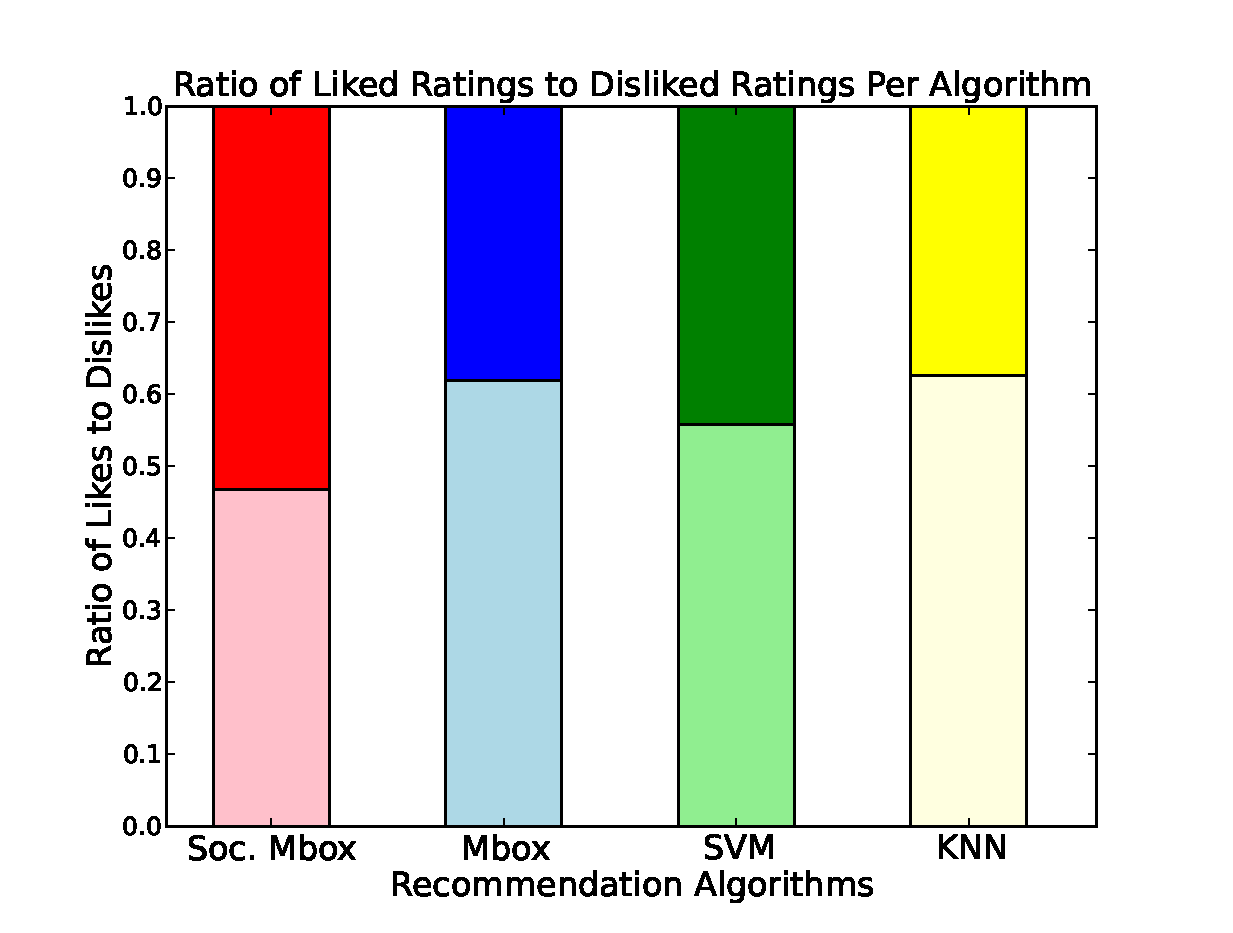
\includegraphics[scale=0.28]{img/live-likes1.eps}}
\subfigure{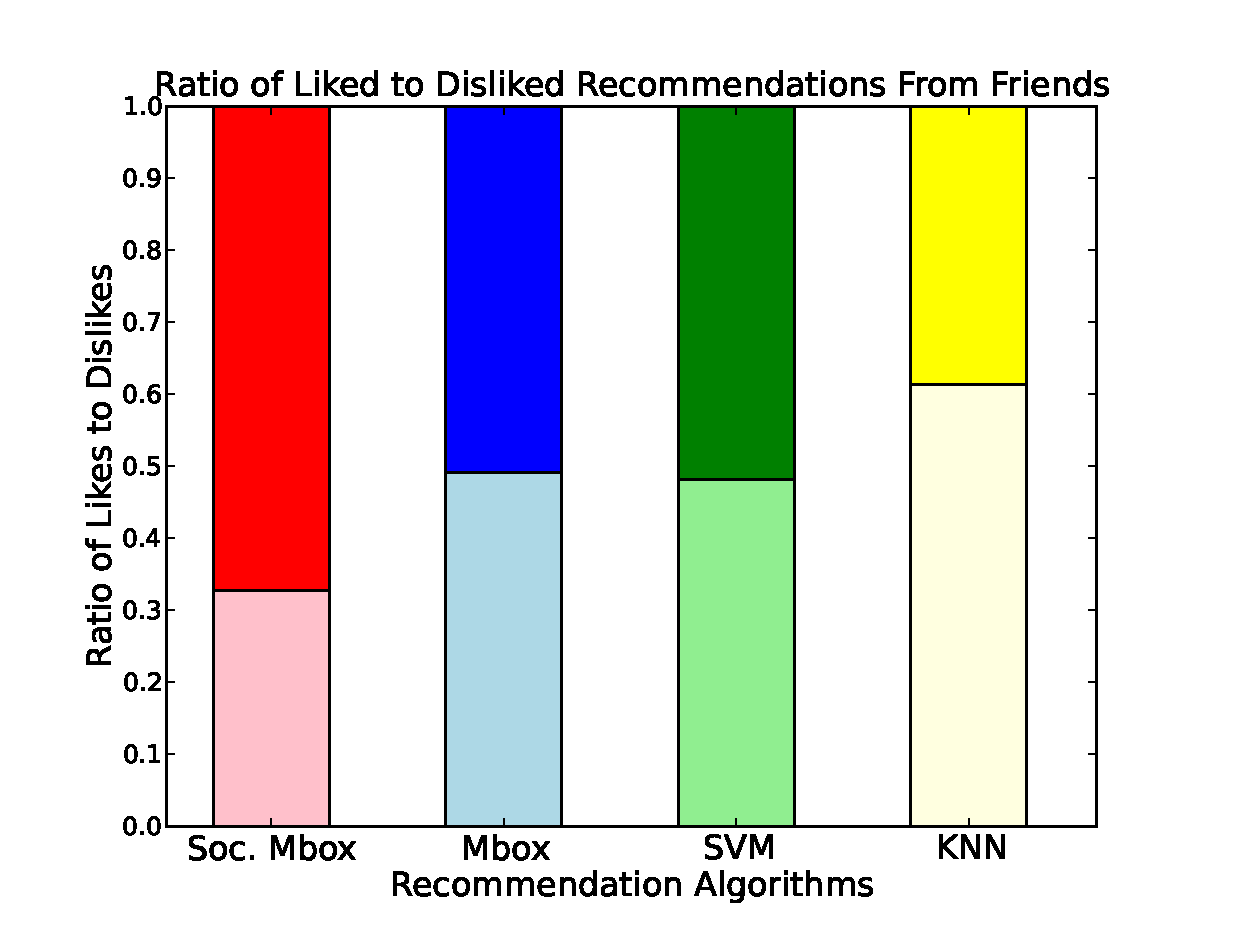
\includegraphics[scale=0.28]{img/live-friend-likes1.eps}}
\subfigure{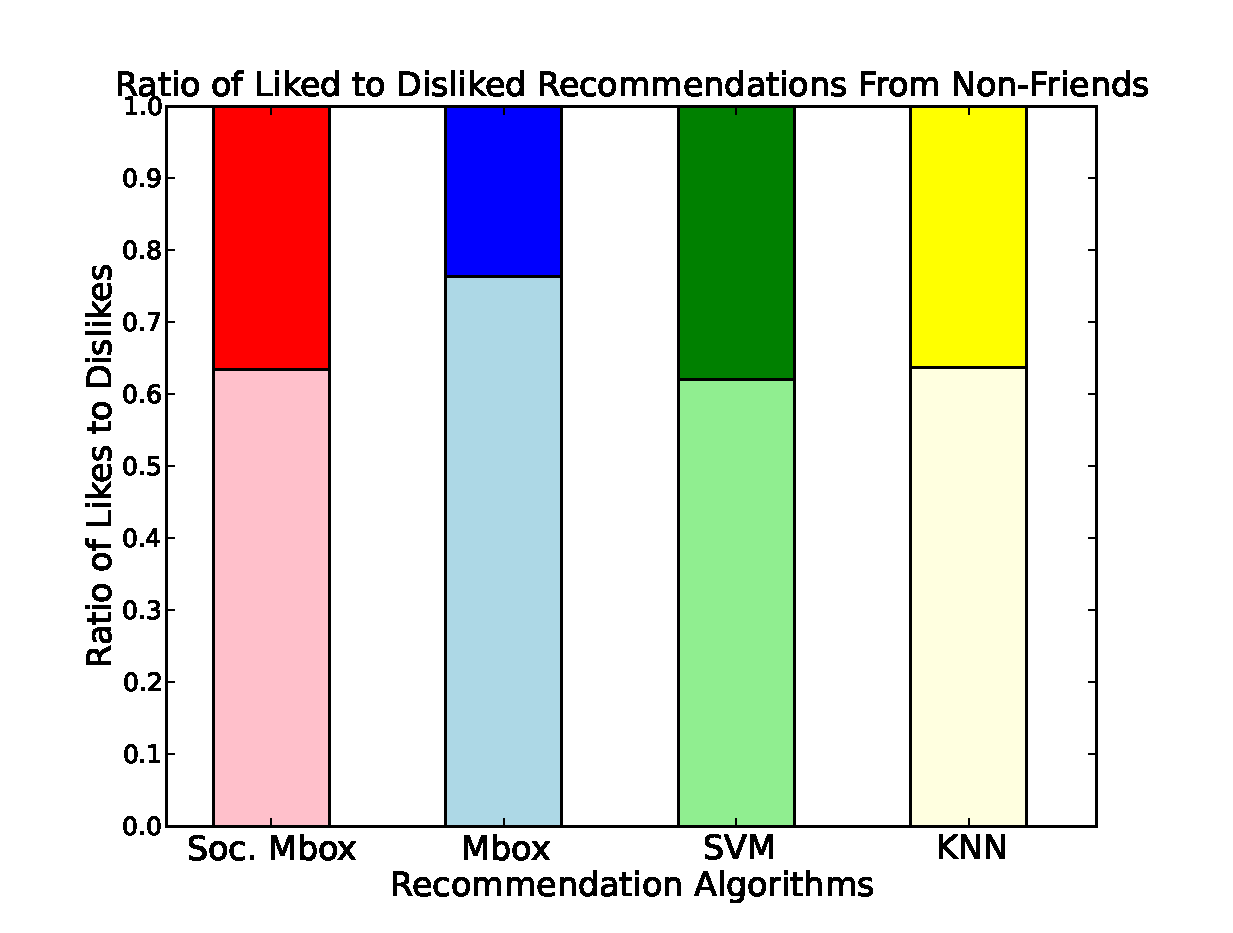
\includegraphics[scale=0.28]{img/live-nonfriend-likes1.eps}}
%\subfigure{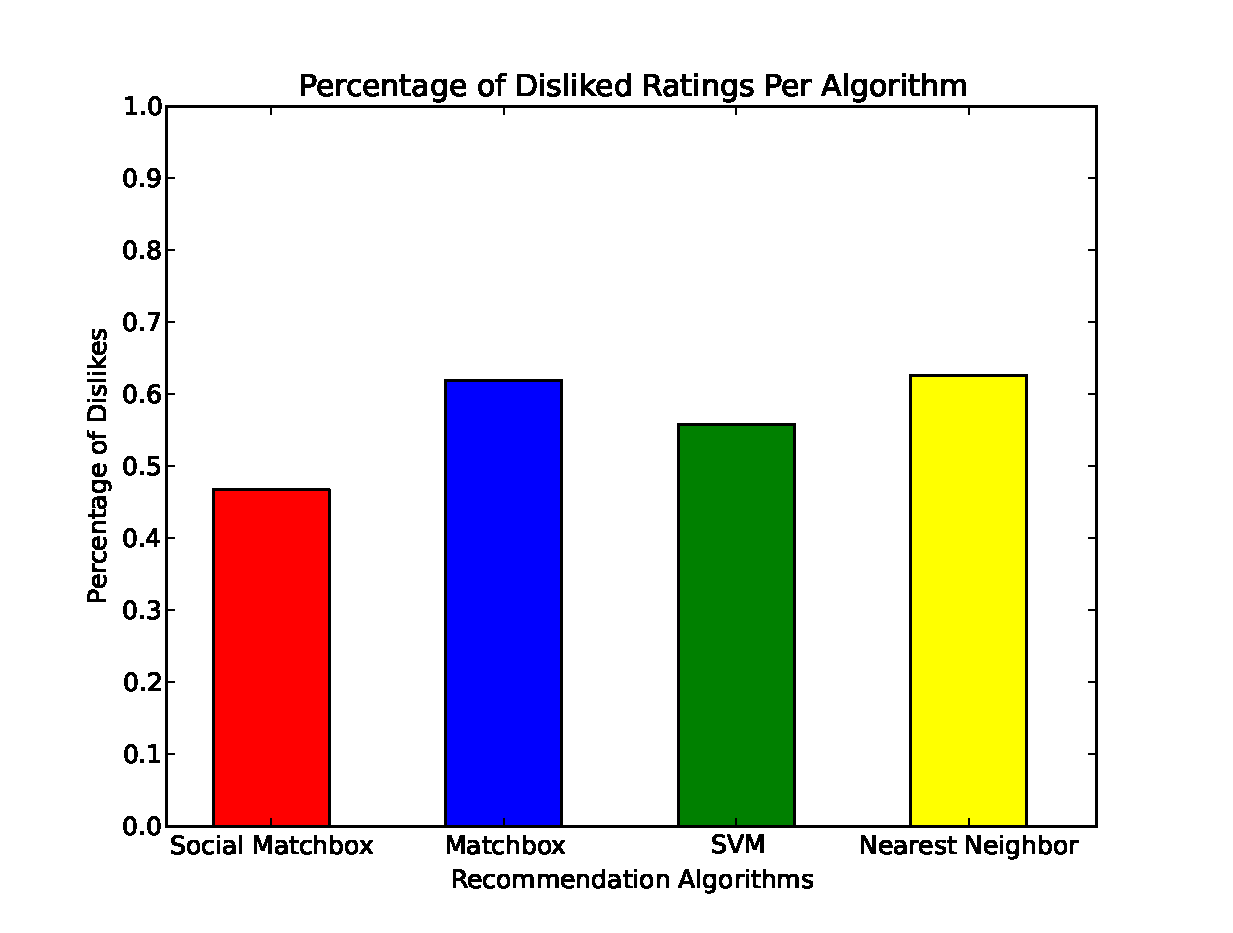
\includegraphics[scale=0.35]{img/live-dislikes1.eps}}
\caption{Results of the online live trials. The percentage of Liked
ratings are stacked on top of the percentage of Disliked ratings per
algorithm. Social Matchbox was found to be the best performing of the
four algorithms evaluated in the first trial.  *** Results of the online
live trials, split between friends and non-friends. The percentage of
Liked ratings are stacked on top of the percentage of Disliked ratings
per algorithm. There is a significant drop in performance between
recommending friend links and recommending non-friend links.}
\label{fig:OnlineResult1}
\end{figure*}

We also look at the algorithms with the results split between friend
links and non-friend links recommendations. Again, the results shown
in Figure~\ref{fig:OnlineFriend1} are the percentage of Like ratings
and the percentage of Dislike ratings per algorithm stacked on top of
each other with the Like ratings on top. As shown in
Figure~\ref{fig:OnlineFriend1}, all four algorithms experienced a
significant performance drop in the ratio of Likes to Dislikes when it
came to recommending non-friend links. This suggests that aside from
Liking or Disliking a link solely from the quality of the link being
recommended, users are also more likely to Like a link simply because
a friend had posted it and more likely to Dislike it because it was
posted by a stranger.

\subsubsection{Summary}

At the end of the first trial, we have observed the following:

\begin{itemize}
\item{Social Matchbox was the best performing algorithm in the live user trial in terms of percentage of likes.}

\item{Social Matchbox received the highest user evaluation scores in the user survey at the end of the user trial.}

\item{Of the various combinations of training and testing data in the offline passive experiment, we found that training on the UNION subset and testing on the APP-USER-ACTIVE-ALL subset best correlated with the results of the live user trial and the user survey. Training on the UNION dataset had advantages compared to training on the other data subsets, namely that it had the large amount of information of the PASSIVE data and the explicit dislikes information of the ACTIVE data.}

\begin{comment}
Explain which offline evaluation correlates with both of these user
feedback metrics... can you briefly explain why?  E.g., training on
UNION gives you explicit negatives, which are crucial (side note,
perhaps not for thesis: except maybe for NN which actually does need
negatives!), and ranking evaluation really requires an accurate list
of likes/dislikes for an accurate ranking metric which can only be had
with the active data}
\end{comment}

\end{itemize}

%%%%%%%%%%%%%%%%%%%%%%%%%%%%%%%
%%%%%%%%%%%%%%%%%%%%%%%%%%%%%%%

\subsection{Second Trial}

For the second online trial, we chose four algorithms again to
randomly split between the LinkR application users. Social Matchbox
was included again as a baseline since it was the best performing
algorithm in the first trial. The distribution count of the algorithms
to the users is shown in Table~\ref{tab:assigned2}

The four SCF algorithms are:

\begin{itemize}
\item{{\bf Social Matchbox (Soc. Mbox)} : Matchbox MF + Social Regularization +  L2 $U$ Regularization + L2 $V$ Regularization}
\item{{\bf Spectral Matchbox (Spec. Mbox)}: Matchbox MF + Social Spectral Regularization + L2 $U$ Regularization + L2 $V$ Regularization}
\item{{\bf Social Hybrid (Soc. Hybrid)}: Hybrid + Social Regularization + L2 $U$ Regularization + L2 $V$ Regularization + L2 $\w$ Regularization}
\item{{\bf Spectral Co-preference (Spec. CP)}: Matchbox MF + Social Co-preference Spectral Regularization + L2 $U$ Regularization + L2 $V$ Regularization}
\end{itemize}

\subsubsection{Online Results}
\label{sec:online2}

The online experiments were switched to the new algorithms on October
13, 2011. For the online results reported here, since the second live
trial is still currently ongoing, we took a snapshot of the data as it
was on October 22, 2011. The algorithms were randomly distributed
among the 103 users who still had the LinkR application installed. The
distribution of the algorithms to the users are show in
Table~\ref{tab:assigned2}


\begin{table}[t!]
\centering
\begin{tabular}{| l | c |}
\hline
{\bf Algorithm} & {\bf Users} \\
\hline
Social Matchbox & 26\\
Spectral Matchbox  & 25 \\
Spectral Co-preference & 27 \\
Social Hybrid & 25 \\
\hline
\end{tabular}
\caption{Number of Users Assigned per Algorithm.}
\label{tab:assigned2}
\end{table}

Results shown in Figure~\ref{fig:online2} are the percentage of Like
ratings and the percentage of Dislike ratings per algorithm stacked on
top of each other with the Like ratings on top.

First thing we note in Figure~\ref{fig:online2} is the decrease in
performance for Social Matchbox, and in fact for all SCF algorithms in
general. Except for Spectral Matchbox, they all received more Dislike
ratings than Like ratings. What we noticed is that of the
recommendations being made in the week that we switched over to the
new algorithms, the majority of the links were about Steve Jobs, who
had died the week previously. We believe that the redundancy and lack
of variety of the links being recommended caused an increase in the
Dislike ratings being given by users on the recommended links. Taking
out the skewed results that follows an unusual event such as this, the
relative algorithm performance was better.

%%%%%%%%%%%%%%%%%%%%%%%%%%%%%%%%%%%%%%%%%%%%%%%%%%%%%%%%%%%%%%%%%%%%%%%%%
\begin{figure*}[t!]
\centering
\subfigure{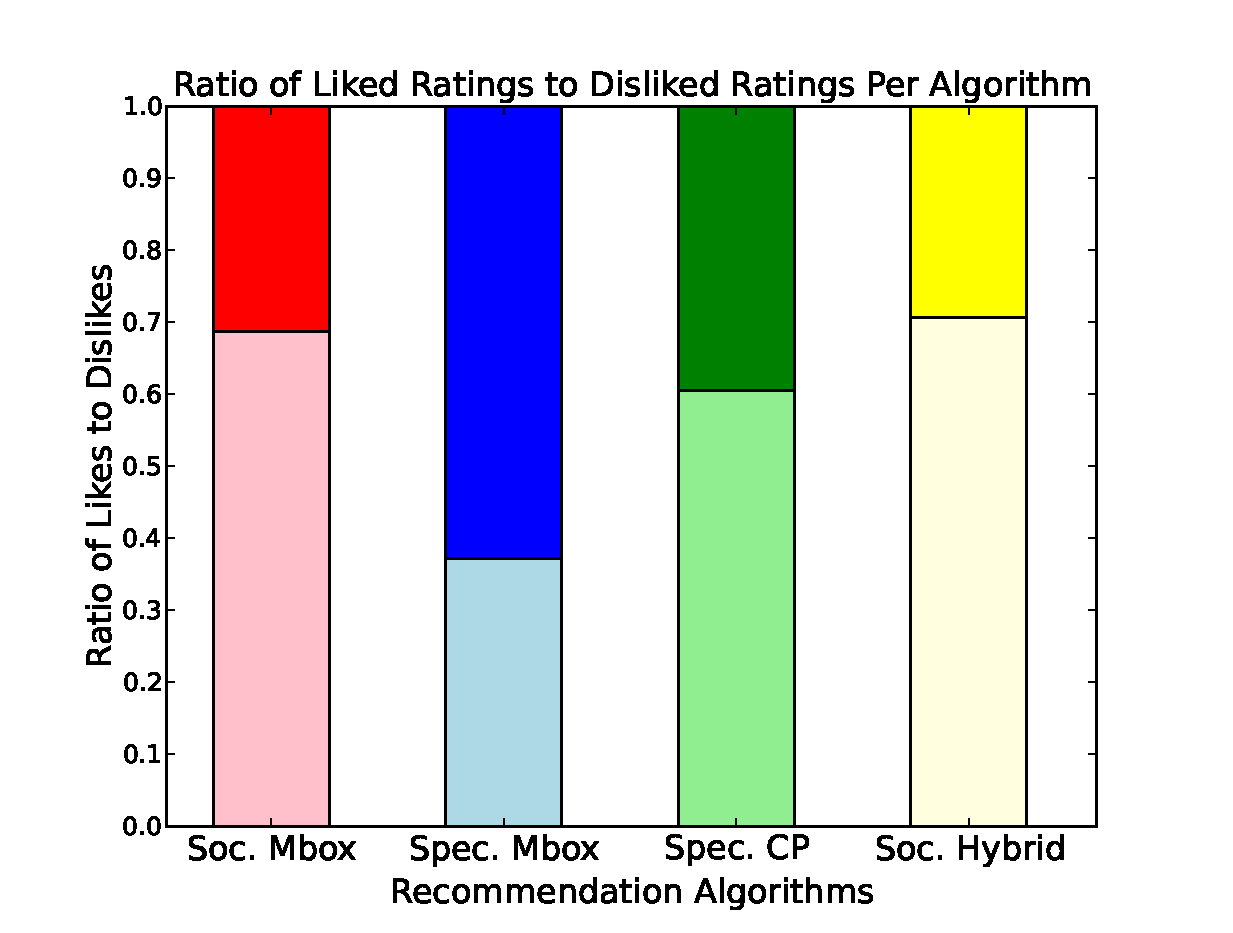
\includegraphics[scale=0.28]{img/live-likes2.eps}}
\subfigure{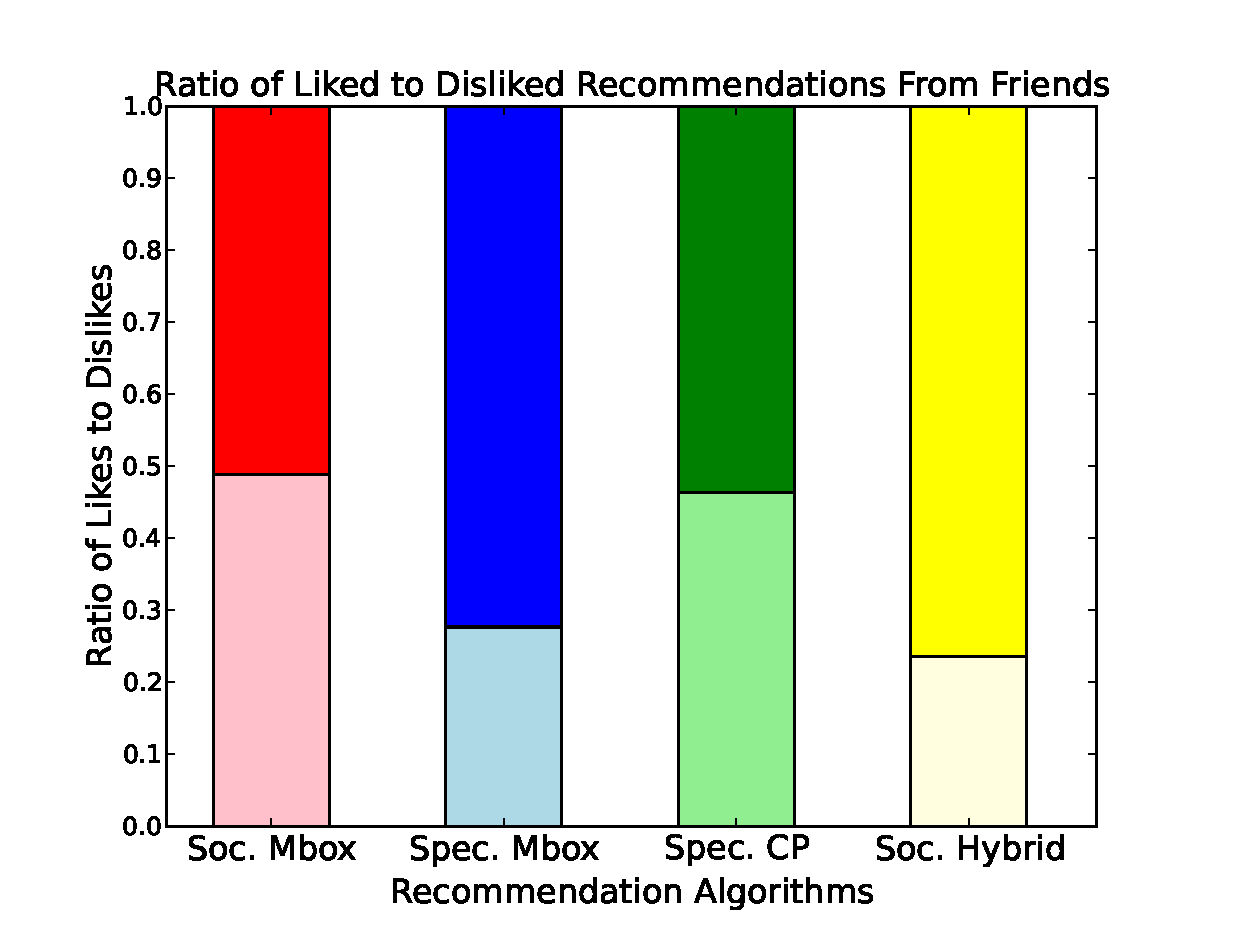
\includegraphics[scale=0.28]{img/live-friend-likes2.eps}}
\subfigure{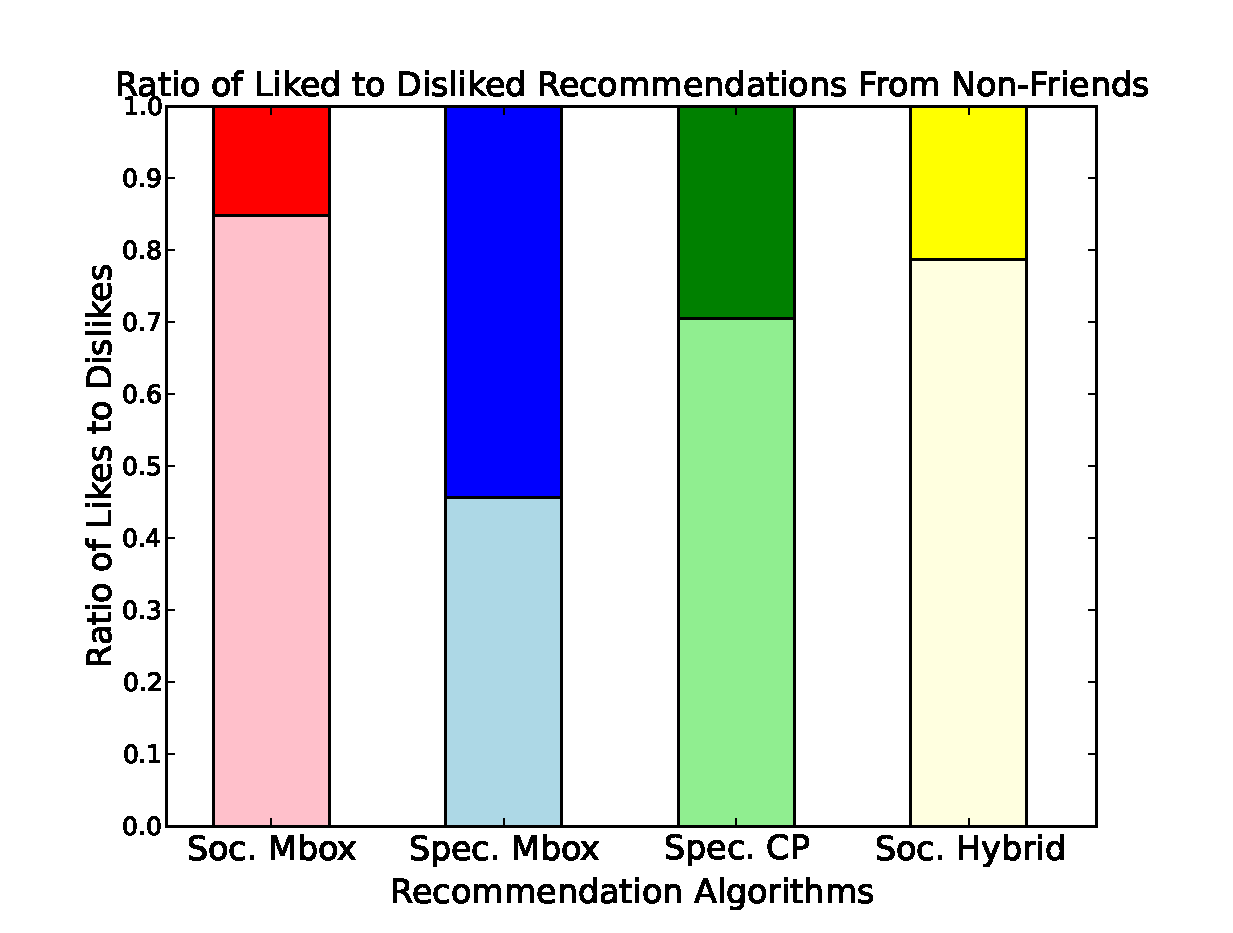
\includegraphics[scale=0.28]{img/live-nonfriend-likes2.eps}}
\caption{Results of online live trials. The percentage of Liked
ratings are stacked on top of the percentage of Disliked ratings per
algorithm. Spectral Matchbox achieved the highest ratio of likes to
dislikes among the four algorithms. Spectral social regularization in
general appears to be a better way to socially regularize compared to
social regularization. *** Results of the online live trials, split
between friends and non-friends. As in the first trial, there is a
significant drop in performance between recommending friend links and
recommending non-friend links.}
\label{fig:online2}
\end{figure*}
%%%%%%%%%%%%%%%%%%%%%%%%%%%%%%%%%%%%%%%%%%%%%%%%%%%%%%%%%%%%%%%%%%%%%%%%%

We again split the results again between friend link recommendations
and non-friend link recommendations, with the results shown in
Figure~\ref{fig:online2} being the percentage of Like ratings and the
percentage of Dislike ratings per algorithm stacked on top of each
other with the Like ratings on top.  As shown
Figure~\ref{fig:online2}, all four algorithms experienced significant
performance drop in the number of likes when it came to recommending
non-friend links. This reflects the results of the first trial.
 
\begin{comment}
Additionally, the differences were more drastic with the two
algorithms that uses the social regularization method: Social Matchbox
and Social Hybrid. This, together with results of the first user
trial, seems to confirm our earlier analysis that aside from Liking or
Disliking a link just from the quality of the links being recommended,
users are also more likely to like a link because a friend had posted
it and more likely to dislike it because it came from a stranger.
\end{comment}

We note the following observations from the results shown in Figures
\ref{fig:online2}:

\begin{itemize}
\item{Compared to the other algorithms, Spectral Matchbox achieved the
best ratio of likes to dislikes as seen, as seen in
Figure~\ref{fig:online2}. Combined with the results for Spectral
Co-preference, Spectral social regularization in general appears to be
a better way to socially regularize compared to social
regularization. This comparison holds even when the results are split
between friend links recommendations and non-friend links
recommendations, as seen in Figure~\ref{fig:online2}.}

\item{When looking at just the friend link recommendations in
Figure~\ref{fig:online2}, Social Hybrid was the best performing
algorithm. This result comes from the user-user information diffusion
among its friends that Social Hybrid learns, which could not be
learned by the other SCF algorithms. Learning information diffusion
thus helps when it comes to building better SCF algorithms.}

\item{Spectral Co-preference didn't do well on friend link
recommendations, however it did better on the non-friend link
recommendations. When it comes to recommending friend links, friend
interaction information coming through social regularizer seems more
important than implicit co-likes information provided by the
co-preference regularizer. When there is no social interaction
information such as with non-friend links, co-preference methods with
its implicit co-likes information appear much better than just vanilla
collaborative filtering at projecting users into subspaces of common
interest.}
\end{itemize}

\subsubsection{Summary}

We summarize the observations made during the second trial:

\begin{itemize}
\item{The social spectral regularization methods generally performed
better in the live user trials, even when the results were split
between friend link recommendations and non-friend link
recommendations.}

\item{Learning information diffusion models helps in SCF, as evidenced
by the strong performance of Social Hybrid when recommending friend
links.}

\item{When there is no social interaction information, learning
implicit co-likes information is better than using plain CF methods.}

\item{The better performance of the social spectral regularization
methods in the live trials were not reflected in the offline
experiments. Perhaps there is a better metric than MAP that correlates
with human preferences.}
\end{itemize}

\subsection{Algorithm Independent Observations}

\subsubsection{Click evidence}

\subsubsection{Impact of Popularity}

\subsubsection{Impact of Interactions}

\subsubsection{Impact of Steve Jobs}

\subsubsection{Impact of Genre}

